% !TEX program  = xelatex
\documentclass{article}
\usepackage[ruled,vlined,linesnumbered]{algorithm2e}
\usepackage{algpseudocode}
\usepackage{amsmath}
\usepackage{amsthm}
\usepackage{graphicx}
\usepackage{subfigure}
\usepackage{float}
\usepackage{amsmath }
\usepackage{amsfonts }
\usepackage{pdfpages}
\usepackage{epsfig}
\usepackage{graphicx}
\usepackage{arydshln}
\usepackage{verbatim}
\usepackage{subfigure}
\usepackage{enumerate}
\usepackage{rotating}
\usepackage{threeparttable}
\usepackage{caption}
\usepackage{epsfig}
\usepackage{cite}
\usepackage{geometry}
\geometry{a4paper, top=2.54cm, bottom=2.54cm, left=3.18cm, right=3.18cm}
\theoremstyle{definition}
\newtheorem{prob}{Problem}
\newtheorem{ans}{Answer}
\usepackage[colorlinks,linkcolor=black]{hyperref}
\linespread{1.2}
\begin{document}
	\title{CS257 Linear and Convex Optimization Homework 10 Solution}
	\author{Kailing Wang 521030910356}
	\date{December 23.2022}
	\maketitle
	\begin{ans}
		~
		
		\begin{enumerate}[(a)]
			\item The approximating equality constrained problem is given by:
			
			$$
			\begin{aligned}
				\underset{\boldsymbol{x} \in \mathbb{R}^{n}}{\min} & \boldsymbol{c}^{T} \boldsymbol{x} - \frac{1}{t} \overunderset{n}{i=1}{\sum}\ln(\boldsymbol{x}_i) \\
				\text { s.t. } & \boldsymbol{A} \boldsymbol{x}=\boldsymbol{b}
			\end{aligned}
			$$
			
			where $t > 0$ is a positive parameter known as the barrier parameter.
			
			\item The gradient of the objective function is given by:
			
			$$ \nabla f(\boldsymbol{x}) = \boldsymbol{c} - \frac{1}{t} \begin{bmatrix} \frac{1}{x_1} \\ \frac{1}{x_2} \\ \vdots \\ \frac{1}{x_n} \end{bmatrix} $$
			
			The Hessian matrix of the objective function is given by:
			
			$$ \nabla^2 f(\boldsymbol{x}) = \frac{1}{t} \begin{bmatrix} \frac{1}{x_1^2} & 0 & \dots & 0 \\ 0 & \frac{1}{x_2^2} & \dots & 0 \\ \vdots & \vdots & \ddots & \vdots \\ 0 & 0 & \dots & \frac{1}{x_n^2} \end{bmatrix} $$
			
			\item Implemented.
			
			\item
			
			$$
			\begin{aligned}
				\min_{\boldsymbol{x} \in \mathbb{R}^{4}} & -3 x_{1}-x_{2} \\
				\text { s.t. } & x_{1}+2 x_{2}+x_{3}=8 \\
				& x_{1}-x_{2}+x_{4}=3 \\
				& x_{1}, x_{2}, x_{3}, x_{4} \geq 0
			\end{aligned}
			$$
			
			Use the implementation of the code to solve and get 
			
			iteration 0: [2 1 4 2]\\
			iteration 1: [4.04872677 1.66477428 0.62167453 0.61599512]\\
			iteration 2: [4.60262517 1.66256807 0.0721469  0.05983965]\\
			iteration 3: [4.66026311 1.66622528 0.00716364 0.00582039]\\
			iteration 4: [4.66595096e+00 1.66663492e+00 6.38994495e-04 5.20316065e-04]\\
			iteration 5: [4.66646946e+00 1.66666880e+00 4.57423071e-05 2.69525426e-05]\\
			iteration 6: [4.66648508e+00 1.66667474e+00 1.65873802e-05 1.51874583e-05]\\
			iteration 7: [4.66649707e+00 1.66667547e+00 1.04225274e-06 1.33128974e-06]\\
			iteration 8: [4.66649731e+00 1.66667536e+00 6.22201973e-07 4.49802772e-07]\\
			iteration 9: [4.66649749e+00 1.66667541e+00 2.23796988e-07 1.89876053e-07]\\
			optimal value: -15.666167890762635			
			
			This answer is correct, anyway.
		\begin{figure}[h]
			\centering
			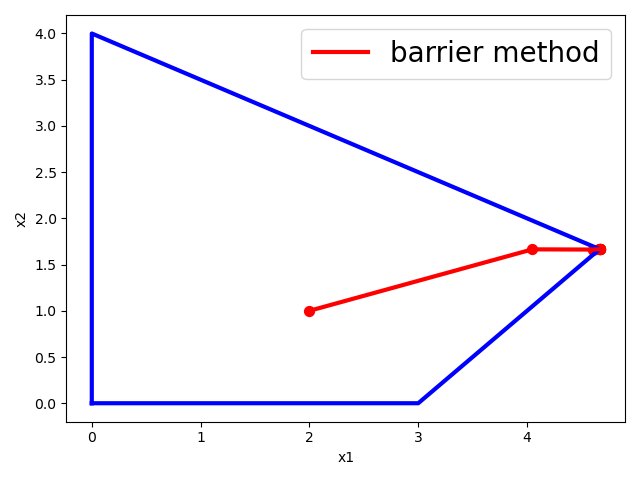
\includegraphics[width=0.5\linewidth]{../p2}
			\caption{barrier method}
		\end{figure}
		\end{enumerate}
	\end{ans}
	
	\begin{ans}
		~
		
		\begin{enumerate}[(a)]
		\item The original LP is like
		$$
		\begin{aligned}
			\min _{\boldsymbol{x} \in \mathbb{R}^{2}} & -3 x_{1}-x_{2} \\
			\text { s.t. } & -x_{1}-2 x_{2} \geq -8 \\
			& -x_{1}+x_{2} \geq -3 \\
			& x_{1} \geq 0 \\
			& x_{2} \geq 0
		\end{aligned}
		$$
		
		We get
		
		$$\left(-\mu_1-\mu_2+\mu_3\right) x_1+\left(-2 \mu_1+\mu_2+\mu_4\right) x_2 \geq-8 \mu_1-3 \mu_2$$
		
		Write it as a dual LP:
		
		$$
		\begin{aligned}
			\max _{\boldsymbol{\mu} \in \mathbb{R}^{4}} & -8 \mu_{1}-3\mu_{2} \\
			\text { s.t. } & -\mu_{1}-\mu_{2}+\mu_3 = -3 \\
			& -2\mu_{1}+\mu_{2}+\mu_4 = -1 \\
			& \mu_{1},\mu_2,\mu_3,\mu_4 \geq 0
		\end{aligned}
		$$
		
		\item Keep the inequality by removing $\mu_3 \text{ and }\mu_4$:
		
		$$
		\begin{aligned}
			\max _{\boldsymbol{\mu} \in \mathbb{R}^{4}} & -8 \mu_{1}-3\mu_{2} \\
			\text { s.t. } & -\mu_{1}-\mu_{2} \leq -3 \\
			& -2\mu_{1}+\mu_{2} \leq -1 \\
			& \mu_{1},\mu_2 \geq 0
		\end{aligned}
		$$
		
		\item The optimal value is $-\frac{47}{3}\approx -15.67$ at $(\frac{4}{3}, \frac{5}{3})$.
		\begin{figure}[h]
			\centering
			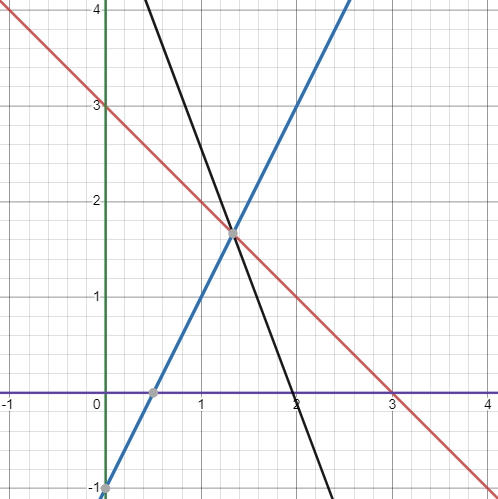
\includegraphics[width=0.3\linewidth]{../graphic}
			\caption{graphic}
		\end{figure}
		
		The graphic is like figure 2.
		
		\item The results is:
		
		iteration 0: [4. 1. 2. 6.]\\
		iteration 1: [1.61522451 1.62970863 0.24474485 0.60066475]\\
		iteration 2: [1.36019967 1.66182412 0.0217291  0.05846118]\\
		iteration 3: [1.33589237 1.66642409 0.00196062 0.00522475]\\
		iteration 4: [1.33368737e+00 1.66684271e+00 1.42149353e-04 3.84674737e-04]\\
		iteration 5: [1.33356991e+00 1.66686590e+00 4.20487722e-05 1.24479483e-04]\\
		iteration 6: [1.33352038e+00 1.66688242e+00 1.75103904e-06 6.29025917e-06]\\
		iteration 7: [1.33352038e+00 1.66688242e+00 1.75103904e-06 6.29025916e-06]\\
		iteration 8: [1.33351848e+00 1.66688359e+00 6.46856320e-07 1.18740179e-06]\\
		iteration 9: [1.33351809e+00 1.66688379e+00 9.41782545e-09 4.11418602e-08]
		dual optimal value: -15.668796087604424
		
		The result is very much the same. 
	 \end{enumerate}
	\end{ans}

	\begin{ans}
		~
		
		\begin{enumerate}[(a)]
			\item 
			$$
			f^{\prime}(x)=\frac{e^x}{2+e^x}\leq 0, x>0
			$$
			
			The optimal value is $f(0)=\ln 3$.
			
			\item The Lagrangian is 
			
			$$
			\mathcal{L}(\boldsymbol{x}, \boldsymbol{\lambda}, \boldsymbol{\mu})=\log \left(2+e^{x}\right)-\mu x
			$$
			$$
			\frac{\partial \mathcal {L}(\boldsymbol{x}, \boldsymbol{\lambda}, \boldsymbol{\mu})}{\partial \boldsymbol{x}}=\frac{e^x}{2+e^x}-\mu
			$$
			$$
			x=\log\frac{2\mu}{1-\mu}, \frac{1}{3}<\mu<1
			$$
			$$
			\begin{aligned}			
			\phi(\boldsymbol{\lambda}, \boldsymbol{\mu})=\inf _{\boldsymbol{x} \in D} \mathcal{L}(\boldsymbol{x}, \boldsymbol{\lambda}, \boldsymbol{\mu})&=\log\frac{2}{1-\mu}-\mu \log\frac{2\mu}{1-\mu}\\
			&=\log 2-\mu\log(2\mu)-(1-\mu)\log(1-\mu)
			\end{aligned}
			$$
			
			When $\mu\geq$1, $\frac{\partial \mathcal {L}(\boldsymbol{x}, \boldsymbol{\lambda}, \boldsymbol{\mu})}{\partial \boldsymbol{x}}<0$, $\phi(\boldsymbol{\lambda}, \boldsymbol{\mu})$=-$\infty$
			
			When $0\leq\mu\leq\frac{1}{3}$, $\frac{\partial \mathcal {L}(\boldsymbol{x}, \boldsymbol{\lambda}, \boldsymbol{\mu})}{\partial \boldsymbol{x}}>0$, $\phi(\boldsymbol{\lambda}, \boldsymbol{\mu})$=$\log 3$
			
			The dual problem is 
			$$
			\begin{aligned}
				\max _{{\mu} \in \mathbb{R}} & \phi(\boldsymbol{\lambda}, \boldsymbol{\mu})\\
				\text { s.t. } & \mu\geq0
			\end{aligned}
			$$
			\item 
			$$
			\phi'(\boldsymbol{\lambda}, \boldsymbol{\mu})=\log\frac{1-\mu}{2\mu}, \frac{1}{3}<\mu<1
			$$
			The optimal value is $\log 3$ at $[0,\frac{1}{3}]$. The strong duality holds.
		\end{enumerate}
	\end{ans}

	\begin{ans}
		~

		\begin{enumerate}[(a)]
			\item The Lagrangian is 
			$$
			\mathcal{L}(\boldsymbol{x}, \boldsymbol{\lambda}, \boldsymbol{\mu})=x_{1}^{2}+x_{2}^{2} + \mu_1(\left(x_{1}-2\right)^{2}+\left(x_{2}-1\right)^{2}-1)+\mu_2(\left(x_{1}-2\right)^{2}+\left(x_{2}+1\right)^{2}-1)
			$$
			
			$$
			\left\{\begin{array}{l}
				\frac{\partial \mathcal{L}}{\partial x_1}=2 x_1+2 \mu_1\left(x_1-2\right)+2 \mu_2\left(x_1-2\right) \\
				\frac{\partial \mathcal{L}}{\partial x_2}=2 x_2+2 \mu_1\left(x_2-1\right)+2 \mu_2\left(x_2+1\right)
			\end{array}\right. 
			$$
			
			$$
			\left\{\begin{array}{l}
				x_1=\frac{2 \mu_1+2 \mu_2}{1+\mu_1+\mu_2} \\
				x_2=\frac{\mu_1-\mu_2}{1+\mu_1+\mu_2}
			\end{array}\right.
			$$
			
			$$
			\phi(\boldsymbol{\lambda}, \boldsymbol{\mu})=\inf _{\boldsymbol{x} \in D} \mathcal{L}(\boldsymbol{x}, \boldsymbol{\lambda}, \boldsymbol{\mu})=\frac{-\left(\mu_1-\mu_2\right)^2+4\left(\mu_1+\mu_2\right)}{1+\mu_1+\mu_2}
			$$	
					
			$$
			\begin{aligned}
				\max_{\boldsymbol{{\mu}} \in \mathbb{R}^2} & \phi(\boldsymbol{\lambda}, \boldsymbol{\mu}) \\
				\text { s.t. } & \mu_1, \mu_2 \geq 0
			\end{aligned}
			$$
			
			\item It's very strange that the feasible set is $\{(2,0)\}$ if we draw the two constraints. The optimal value of the original problem is 4. 
			
			$$\frac{\mathrm{d}}{\mathrm{d}\mu_1}\frac{-\left(\mu_1-\mu_2\right)^2+4\left(\mu_1+\mu_2\right)}{1+\mu_1+\mu_2} = \frac{\left(-2\mu_1+2\mu_2+4\right)\left(1+\mu_1+\mu_2\right)-\left(-\left(\mu_1-\mu_2\right)^2+4\left(\mu_1+\mu_2\right)\right)}{\left(1+\mu_1+\mu_2\right)^2}$$
			
			$$\frac{\mathrm{d}}{\mathrm{d}\mu_2}\frac{-\left(\mu_1-\mu_2\right)^2+4\left(\mu_1+\mu_2\right)}{1+\mu_1+\mu_2} = \frac{\left(2\mu_1-2\mu_2+4\right)\left(1+\mu_1+\mu_2\right)-\left(-\left(\mu_1-\mu_2\right)^2+4\left(\mu_1+\mu_2\right)\right)}{\left(1+\mu_1+\mu_2\right)^2}$$
			
			The gradient is always positive when $\mu_1\geq0 \text{ and }\mu_2\geq0$. The optimal value 4 dose not exist, or to say is at $\boldsymbol{\mu}=(+\infty, +\infty)$. Strong duality holds if we accept infinity.
			
			\item The feasible set is a single point while the two restriction functions are not affine, so the Slater’s condition doesn’t hold.
			
			\item The dual optimal value is at $\boldsymbol{\mu}=(+\infty, +\infty)$ which cannot be obtained by any point. It's easy to find the stationarity of KKT is not satisfied because we assume the dual solution can be obtained by a certain point. 
		\end{enumerate}
	\end{ans}

	\begin{ans}
		~
		
		\begin{enumerate}[(a)]
			\item 
			$$
			\left\{\begin{array}{l}
				\frac{\partial \mathcal{L}}{\partial x_1}=5 x_1^4-\mu=0 \\
				\frac{\partial \mathcal{L}}{\partial x_2}=5 x_2^4-\mu=0
			\end{array}\right.
			$$
			$$
			\left\{\begin{array}{l}
				x_1=\sqrt[4]{\frac{\mu}{5}} \\
				x_2=\sqrt[4]{\frac{\mu}{5}}
			\end{array}\right.
			$$
			$$
			\phi(\mu)=\inf _{\boldsymbol{x}\in \boldsymbol{D}} \mathcal{L}=2(\frac{\mu}{5})^{\frac{5}{4}}+\mu(1-2(\frac{\mu}{5})^{\frac{1}{4}}), \mu \geq 0
			$$
			\item 
			$$
			\phi'(\mu)=\inf _{\boldsymbol{x}\in \boldsymbol{D}} \mathcal{L}=\frac{5}{2}(\frac{\mu}{5})^{\frac{1}{4}}+1-2(\frac{\mu}{5})^{\frac{1}{4}}-\mu\cdot\frac{1}{2}(\frac{\mu}{5})^{\frac{1}{4}} , \mu \geq 0
			$$
			
			The optimal value $\phi^*=\frac{1}{16}$ is obtained at $\mu=\frac{5}{16}$
			
			\item
	
			At $x_1=x_2=\frac{1}{2}, \mu=\frac{5}{16}$, the KKT conditions:
			$$
			\begin{aligned}
				1-x_1-x_2=0 \leq 0 \\
				\mu=\frac{5}{16} \geq 0 \\
				\nabla_{\boldsymbol{x}} L=\overrightarrow{0} \\
				\mu\left(1-x_1-x_2\right)=0
			\end{aligned}
			$$
			
			and f is convex. Thus $\frac{1}{16}$ is the prime optimal value. 
			
			\item
			The Lagrangian is
			$$
			\mathcal{L}=x_1^5+x_2^5-\mu_1\left(x_1+x_2-1\right)-\mu_2 x_1-\mu_3 x_2
			$$
			
			$\boldsymbol{D}=\mathbb{R}^2$, we have the dual function
			$$
			\phi(\mu)=\inf _{\boldsymbol{x}} \mathcal{L}=-\infty
			$$
			Strong duality does not hold.
		\end{enumerate}
	\end{ans}
\end{document}